%#! platex thesis.tex

%======================================================================
\chapter{実装}
\label{cha:imple}
本章では,データ収集の方法について説明し,SRP手法とLSTMを用いたオンライン手書き医療用語認識手法の実装について説明する.
%----------------------------------------------------------------------
\section{データ収集}
\label{sec:collection}
本研究では,学習に使用したいデータがオープンソースで存在していないため,独自でデータ収集を行う必要があった.以下収集したデータの内容,収集手順を説明する.

\begin{figure}[tb]
 \begin{center}
  \resizebox{\columnwidth}{!}{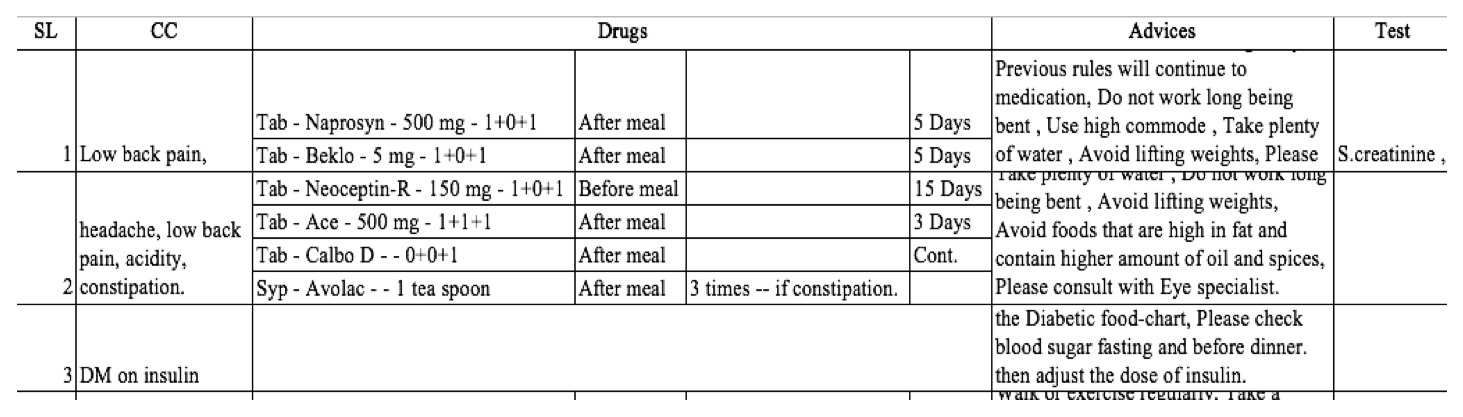
\includegraphics{img/corpus.eps}}
  \caption{PHCの処方箋データ(一部)}
  \label{corpus}
\end{center}
\end{figure}

\begin{figure}[tb]
  \begin{center}
     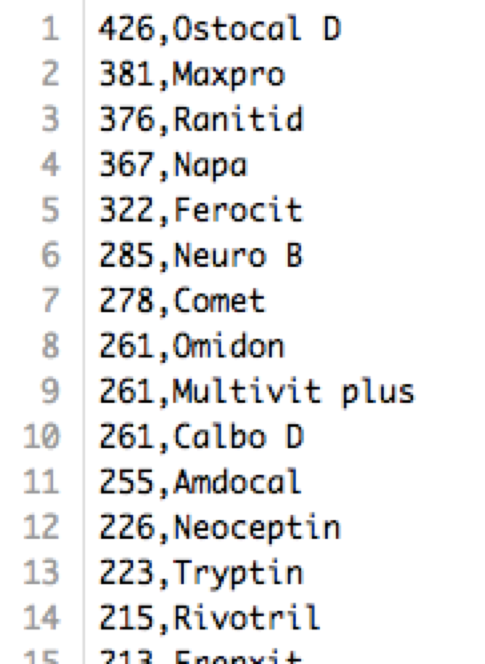
\includegraphics[keepaspectratio,scale=0.5]{img/corpus_example.png}\\
  \end{center}
 \caption{薬名欄のコーパス(一部)}
 \label{corpus_example}
\end{figure}

\subsection{医療用語コーパス}
\label{ssec:corpus}
過去の処方箋データから医療用語コーパスを作成した.コーパスとは,言語を分析するための基礎資料として書き言葉や話し言葉の資料を収集し,研究用の情報を付与したものである.本研究では医療用語の手書き認識を行う.そこで \ref{sec:background}節で述べたPHCの過去の処方箋データからコーパスを作成し,それを機械学習の正解データとして用いた. \textbf{図~\ref{corpus}}にコーパス作成に使用したPHCの過去の処方箋データを示す.8324名分の過去の処方箋データは,それぞれの欄が症状,薬名などに分けられる.\textbf{図~\ref{corpus_example}}に本研究で作成したコーパスの例として,薬名欄のコーパスの一部を示す.それぞれの欄において全ての文を1単語ごとに区切り,単語の出現回数を数えて単語を並び替えた.

本研究では薬名欄に頻出する単語(360語,英語)と医者からのアドバイス欄に頻出する単語(120語,バングラ語)を用いてコーパスを作成し,データ収集を行った.

\begin{figure}[tb]
 \begin{center}
  \resizebox{\columnwidth}{!}{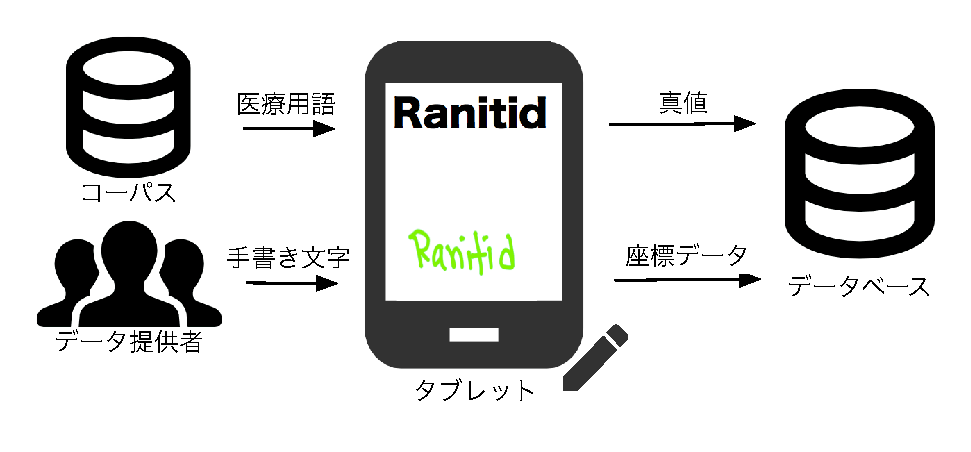
\includegraphics{img/app_structure.eps}}
  \caption{データ収集アプリの構造}
  \label{app_structure}
\end{center}
\end{figure}
%
%----------------------------------------------------------------------
\subsection{データ収集用アプリ}
\label{ssec:app}
\textbf{図~\ref{app_structure}} にデータ収集用アプリの構造を示す.オンライン手書き文字を収集するため,株式会社CodeNext\cite{codenext}にAndroidアプリの作成を依頼した.このアプリは\ref{ssec:corpus}項で作成したコーパスから単語を1語ずつ表示し,データ提供者は表示された単語をタブレットに手書きで記入する.手書きされた文字は正解データとともにデータベースに保存される.\textbf{図~\ref{app_image}}にアプリ画面のイメージ図を示す.

\begin{figure}[tb]
 \begin{center}
  \resizebox{\columnwidth}{!}{\includegraphics{img/app_image.eps}}
  \caption{データ収集アプリイメージ図}
  \label{app_image}
\end{center}
\end{figure}

\section{使用機器}
\label{sec:machine}
\textbf{図~\ref{equipments}}に使用機器を示す.データ収集用のタブレットは Samsung 社の Galaxy Tab S3 を用いた.1つのタブレットに1つのスタイラスペンが付属している.機械学習には NVIDIA社の GeForce 1080 が1枚搭載された デスクトップ PC を用いた.\textbf{~\tablename~\ref{tab:spec}}に実装環境を示す.

\begin{figure}[tb]
 \begin{center}
  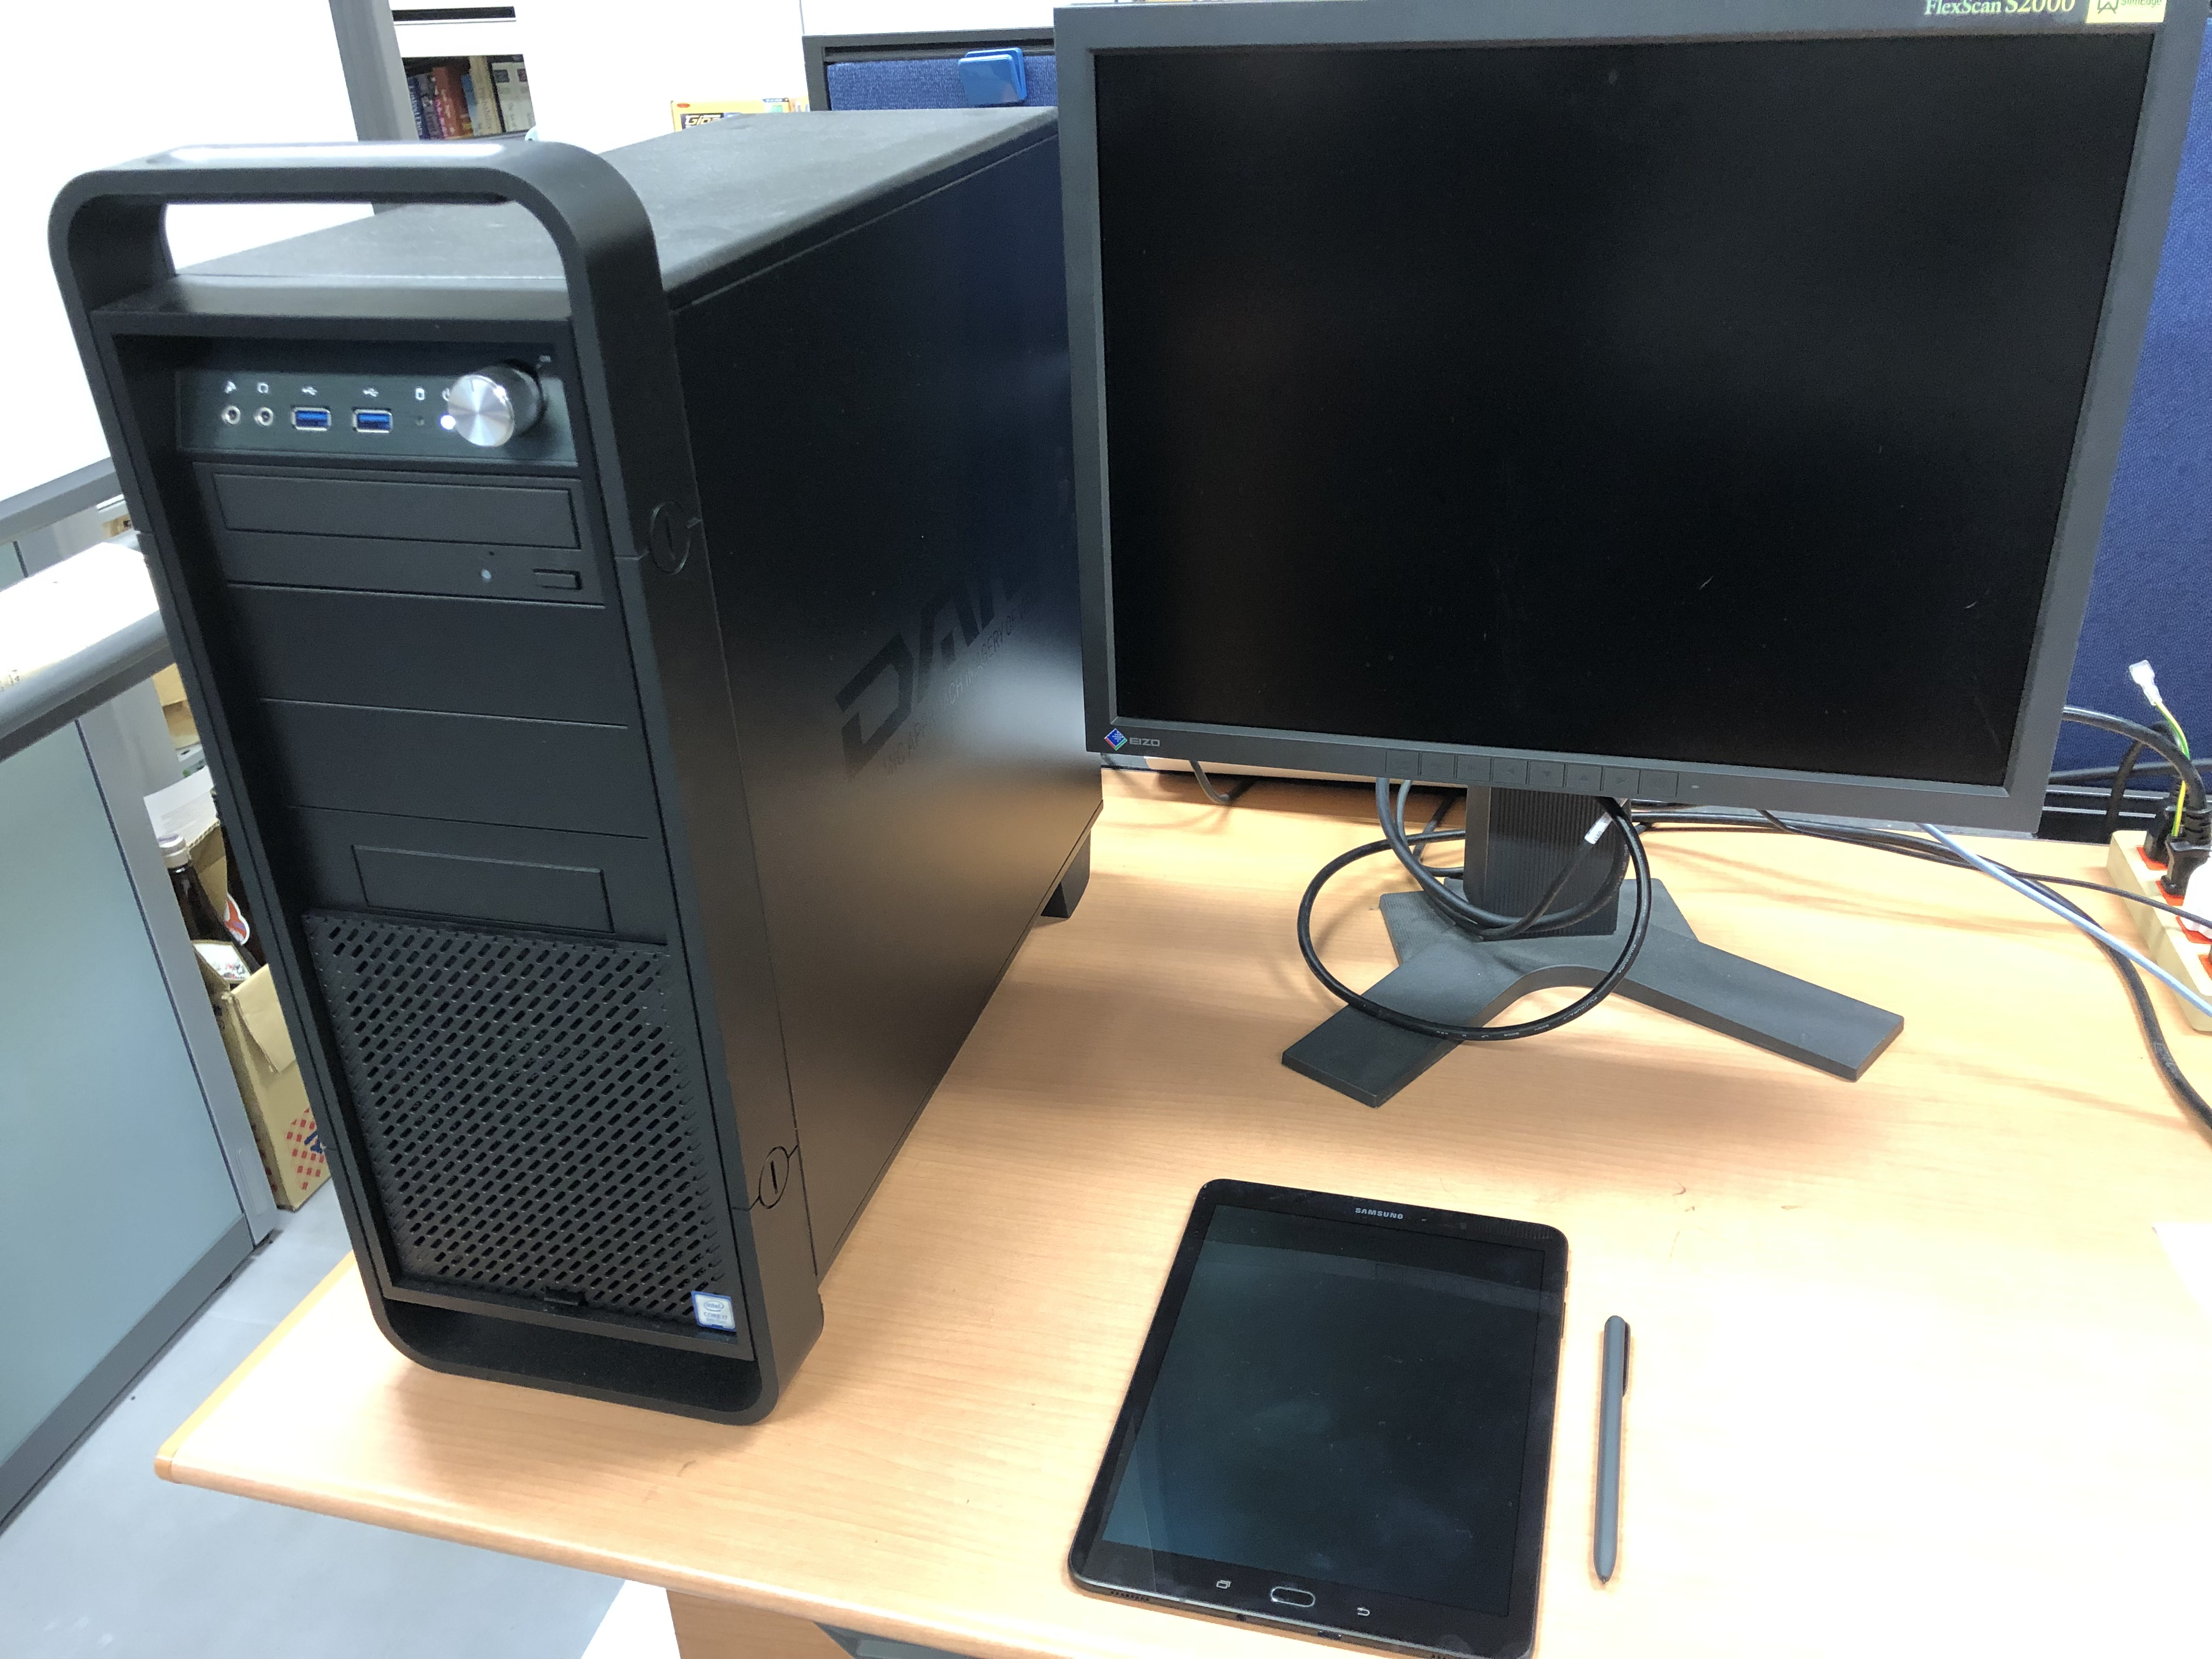
\includegraphics[keepaspectratio, scale=0.1]{img/equipments.png}
  \caption{使用機器}
  \label{equipments}
\end{center}
\end{figure}

\begin{table}[bt]
 \centering
 \caption{実装環境}
 \label{tab:spec}
 \begin{tabular}{ll}\Hline
  OS & \texttt{Ubuntu 16.04}\\
  GPU & \texttt{NVIDIA GeForce 1080}\\
  メモリ & \texttt{8GB}\\
  プロセッサ & \texttt{3.70GHz Intel Core i7-8000K}\\
  \hline
  タブレット & \texttt{Samsung Galaxy Tab S3}\\
 \Hline
 \end{tabular}
\end{table}

\section{学習モデル構造}
\textbf{図~\ref{layers}}に本研究で用いた学習モデルの構造を示す.文献\cite{zhang18:drawing}を参考に作成し,実装にはpythonのニューラルネットワークライブラリであるKeras\cite{keras}を用いた.本研究で用いるデータはデータ長が一定ではないため,データの後ろを$0$でパディングすることでデータ長最大の値である$260$に揃え,学習の入力とした.LSTM層の出力次元数は$300$に設定し,プールサイズの値の平均値をそれぞれ出力するプーリング層を配置した.その後パラメータの数を増やすために全結合層を配置した.なお,過学習を防ぐためプーリング層と全結合層の間にドロップアウト\cite{dropout}をそれぞれ$0.3$の割合で設定した.

\begin{figure}[tb]
 \centering
  \begin{tabular}{c}
    \begin{minipage}[b]{0.7\hsize}
     \centering
     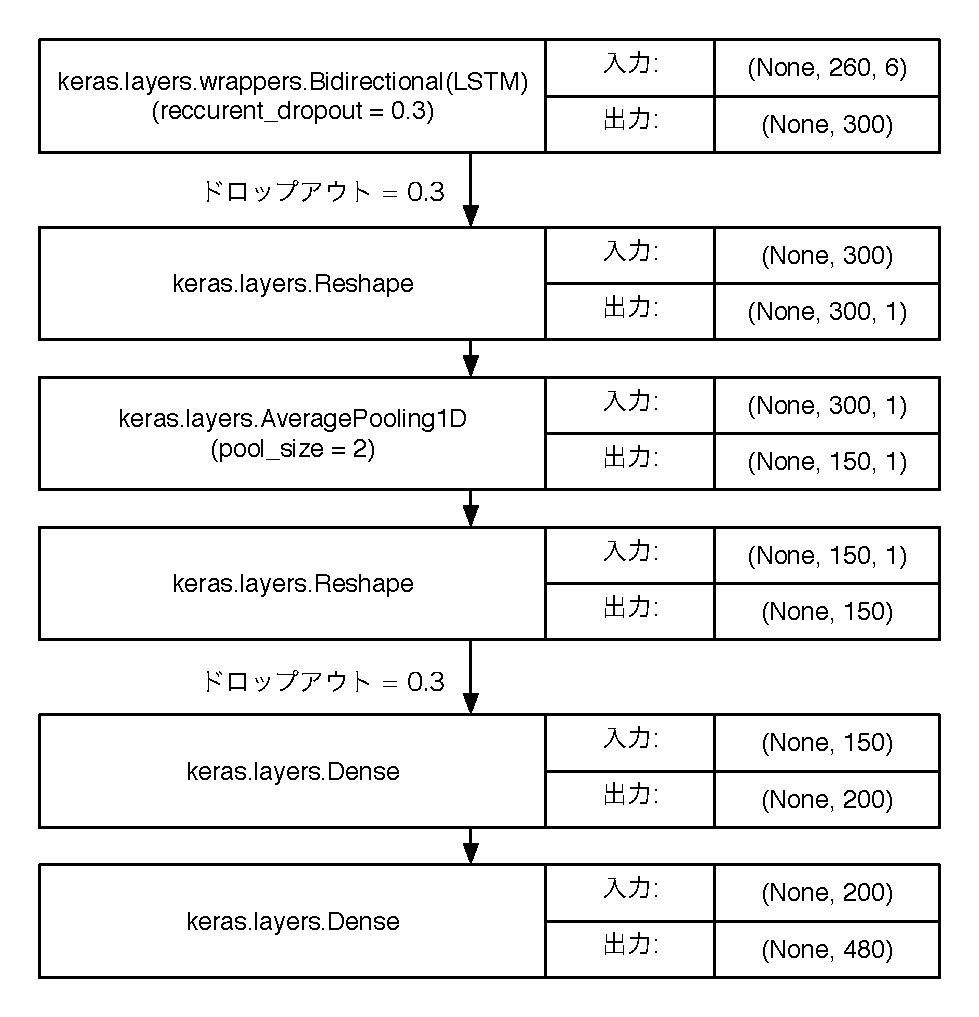
\includegraphics[keepaspectratio,scale=0.7]{img/layers.eps}\\
    \end{minipage}
  \end{tabular}
 \caption{層の構成}
 \label{layers}
\end{figure}

% 以下はRefTeX用
%%% Local Variables:
%%% mode: yatex
%%% TeX-master: "thesis"
%%% End:
